\documentclass[fr]{../../../../../../eplexam}

\hypertitle{Théorie des graphes (MIN)}{5}{INMA}{1961}{2017}{Janvier}
{Etudiants MAP de 2017}
{Vincent Blondel et Jean-Charles Delvenne}

\section{}
Minerva McGonnagall, directrice-adjointe de l’école de Poudlard, est chargée de faire les horaires
et ce n’est pas une mince affaire. En effet, une certaine Hermione Granger a décidé de
suivre l’ensemble des cours. En tenant compte des horaires bien remplis des professeurs et après
soustraction du tronc commun, voici les cours pour lesquels un horaire reste à attribuer : 
\begin{itemize}
	\item Arithmancie : Lu 16h, Je 8h, Ve 8h
	\item Botanique : Lu 16h, Ma 16h, Je 16h, Ve 8h, Ve 16h
	\item Divination : Lu 8h, Ma 8h, Je 16h
	\item Etudes des Moldus : Ma 16h, Je 8h
	\item Histoire de la Magie : Lu 16h, Ma 16h
	\item Métamorphose : Lu 16h, Je 8h
	\item Runes antiques : Lu 8h, Ma 8h, Ve 8h, Ve 16h
	\item Soins aux Créatures Magiques : Lu 16h, Ma 16h
\end{itemize}

Prof. McGonagall, impuissante face à ce problème, demande à Septima Vector, professeur
d’Arithmancie, de préparer un horaire permettant à Mlle Granger d’assister à tous les cours.
Le Département des Mystères, au pire, est prêt à louer un retourneur de temps capable de
vous ramener deux heures (la durée d’un cours) en arrière, à la condition que l’élève l’utilise le
moins possible.\\
Septima Vector pourra-t-elle remettre un horaire satisfaisant ? Dans le cas contraire, combien
de fois par semaine au minimum Mlle Granger devra-t-elle utiliser le retourneur de temps ? 

\begin{solution}

 On peut remarquer qu'Histoire de la magie et Soins aux créatures magiques ont exactement les mêmes horaires. Cela a comme conséquence que Etudes des moldus et Métamorphose doivent être suivis en même temps. \\ Hermione aura donc besoin d'utiliser le retourner 1 fois par semaine. \\
Une proposition d'horaire : 
\begin{itemize}
	\item Soins : Ma 16h
	\item Histoire : Lu 16h
	\item Etude ET Métamorphose : Je 8h
	\item Arithmancie : Ve 8h
	\item Botanique : Je 16h
	\item Divinatio : Lu 8h
	\item Runes : Ve 16h
\end{itemize}

Plus formellement, on crée un graphe biparti avec d'un côté les cours et de l'autre côté les plages horaires. On relie les cours aux plages horaires possibles. Il faut alors trouver un couplage maximum. S'il n'est pas parfait, il faudra utiliser le retourneur de temps autant de fois qu'il y a de cours qui n'appartiennent pas au couplage.

\begin{solfig}{c}{Graphe biparti}
	\centering
	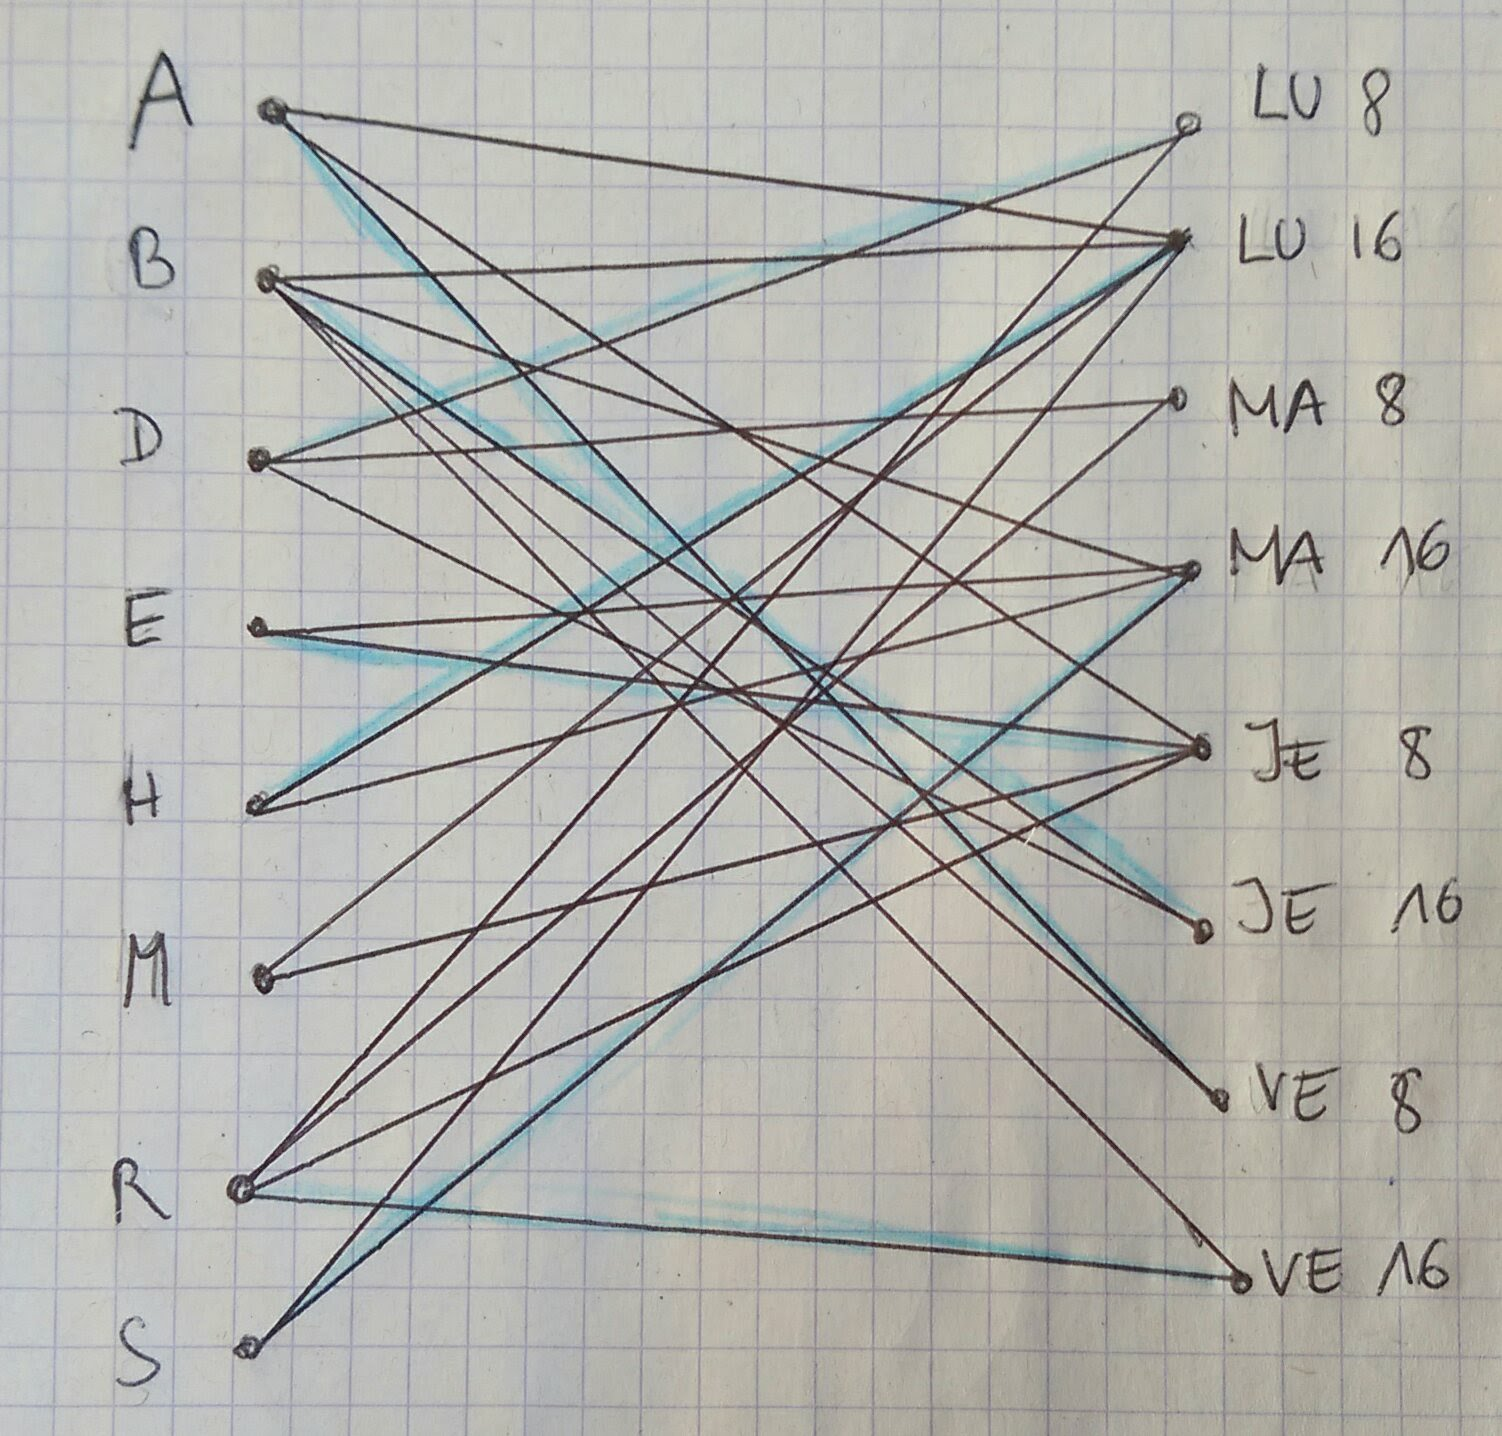
\includegraphics[width=0.7\textwidth]{IMAG0297_1.jpg}
\end{solfig}

\end{solution}

\section{}
\begin{enumerate}
	\item Démontrez que dans une suite de 5 nombres réels distincts, se trouve une sous-suite croissante
	de 3 éléments, ou une sous-suite décroissante de 3 nombres. Par exemple la suite 12, 3, 9, 7, 5 contient la sous-suite décroissante 12, 9, 7.
	\item Démontrez que pour tous les naturels $r$, $s$, il existe un nombre fini $f(r, s)$ tel que toute suite de $f(r, s)$ réels distincts contient une sous-suite croissante de $r$ éléments ou une sous-suite décroissante de $s$ éléments.
\end{enumerate}

\nosolution




\section{}
On sait que le nombre chromatique d’un graphe simple G est borné par $\chi(G) \leq degmax(G)+1$.\\

Illustrez cette borne pour l’étoile à $n$ noeuds (qui est un arbre avec une racine et $n − 1$ feuilles). Est-ce une bonne borne, à votre avis ?

\begin{solution}

Avec une étoile à 6 noeuds, $dmax = 5 $, donc on peut utiliser 6 couleurs. Cette borne est ici très mauvaise, 2 couleurs suffisent !

\begin{solfig}{c}{1e sous question de la question 3}
	\centering
	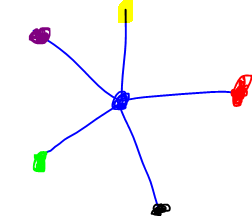
\includegraphics[scale=0.75]{jan2017MinQ3.PNG}
	\label{fig:univerise}
\end{solfig}

\end{solution}

\section{}
Vrai ou faux.

\begin{enumerate}
	\item Tout graphe connexe à $n$ noeuds et $n + 1$ arêtes est planaire. 
	
	\item  Toute représentation dans le plan d’un graphe simple à $3 \leq n$ noeuds et $m$ arêtes comporte au moins $m - 3n + 6$ croisements d’arêtes.
	
	\item Il existe un graphe planaire qui est 6-connexe. 
	
	\item Tout arbre G possède au moins $degmax(G)$ feuilles.
	
	\item Si je dispose 120 pièces de 1 euro à plat sur la table, éventuellement contigües, je peux en trouver 30 non-contigües deux à deux.
	
\end{enumerate}

\begin{solution}
	
\begin{enumerate}
	\item VRAI : pour que le graphe soit connexe, on doit utiliser $n-1$ arêtes, il en reste 2. Donc, c'est impossible d'obtenir $K_5$ ou $K_{3,3}$ en rajoutant seulement 2 arêtes à une chaine, c'est un graphe planaire.
	
	\item VRAI ?
	
	\item FAUX : $K_6$ contient $K_5$.
	
	\item VRAI.
	
	\item VRAI: Tout graphe planaire possède un coloriage propre de 4 couleurs, alors il existe d'office un ensemble indépendant d'au moins 30 monnaies, car la somme des quatre ensembles indépendants doit être égale à 120.
	
\end{enumerate}

\end{solution}

\end{document}
